%% 
%% Copyright 2007-2025 Elsevier Ltd
%% 
%% This file is part of the 'Elsarticle Bundle'.
%% ---------------------------------------------
%% 
%% It may be distributed under the conditions of the LaTeX Project Public
%% License, either version 1.3 of this license or (at your option) any
%% later version.  The latest version of this license is in
%%    http://www.latex-project.org/lppl.txt
%% and version 1.3 or later is part of all distributions of LaTeX
%% version 1999/12/01 or later.
%% 
%% The list of all files belonging to the 'Elsarticle Bundle' is
%% given in the file `manifest.txt'.
%% 
%% Template article for Elsevier's document class `elsarticle'
%% with numbered style bibliographic references
%% SP 2008/03/01
%% $Id: elsarticle-template-num.tex 272 2025-01-09 17:36:26Z rishi $
%%
\documentclass[preprint,12pt]{elsarticle}

%% Use the option review to obtain double line spacing
%% \documentclass[authoryear,preprint,review,12pt]{elsarticle}

%% Use the options 1p,twocolumn; 3p; 3p,twocolumn; 5p; or 5p,twocolumn
%% for a journal layout:
%% \documentclass[final,1p,times]{elsarticle}
%% \documentclass[final,1p,times,twocolumn]{elsarticle}
%% \documentclass[final,3p,times]{elsarticle}
%% \documentclass[final,3p,times,twocolumn]{elsarticle}
%% \documentclass[final,5p,times]{elsarticle}
%% \documentclass[final,5p,times,twocolumn]{elsarticle}

%% For including figures, graphicx.sty has been loaded in
%% elsarticle.cls. If you prefer to use the old commands
%% please give \usepackage{epsfig}

%% The amssymb package provides various useful mathematical symbols
\usepackage{amssymb}
%% The amsmath package provides various useful equation environments.
\usepackage{amsmath}
%% The amsthm package provides extended theorem environments
%% \usepackage{amsthm}
\usepackage{array}
\usepackage{tabularx}
\usepackage{booktabs}
%% The lineno packages adds line numbers. Start line numbering with
%% \begin{linenumbers}, end it with \end{linenumbers}. Or switch it on
%% for the whole article with \linenumbers.
%% \usepackage{lineno}

\journal{BioSystems}

\begin{document}

\begin{frontmatter}

%% Title, authors and addresses

%% use the tnoteref command within \title for footnotes;
%% use the tnotetext command for theassociated footnote;
%% use the fnref command within \author or \affiliation for footnotes;
%% use the fntext command for theassociated footnote;
%% use the corref command within \author for corresponding author footnotes;
%% use the cortext command for theassociated footnote;
%% use the ead command for the email address,
%% and the form \ead[url] for the home page:
%% \title{Title\tnoteref{label1}}
%% \tnotetext[label1]{}
%% \author{Name\corref{cor1}\fnref{label2}}
%% \ead{email address}
%% \ead[url]{home page}
%% \fntext[label2]{}
%% \cortext[cor1]{}
%% \affiliation{organization={},
%%             addressline={},
%%             city={},
%%             postcode={},
%%             state={},
%%             country={}}
%% \fntext[label3]{}

\title{Information Evolution by Bayesian Assembly}

%% use optional labels to link authors explicitly to addresses:
%% \author[label1,label2]{}
%% \affiliation[label1]{organization={},
%%             addressline={},
%%             city={},
%%             postcode={},
%%             state={},
%%             country={}}
%%
%% \affiliation[label2]{organization={},
%%             addressline={},
%%             city={},
%%             postcode={},
%%             state={},
%%             country={}}

\author{Dan Adler} %% Author name

%% Author affiliation
\affiliation{organization={BNY},%Department and Organization
            country={US}}

%% Abstract
\begin{abstract}
%% Text of abstract
The emergence of complexity and information is a fundamental question spanning disciplines from physics to biology and computation. Although traditional approaches often describe information as an emergent property, they leave unresolved how it dynamically arises from purely abiotic processes. This paper introduces Bayesian Assembly (BA) systems, an abstract framework that models the evolution of patterns through probabilistic interactions and stability-driven selection. By abstracting away specific physical laws, BA systems offer a universal mechanism for generating order and information. Extending the principles of Assembly Theory (AT), BA systems emphasize forward dynamics, where selection pressures favor stable configurations that persist and interact more frequently. These dynamics provide a basis for understanding processes that could underlie the transition from abiotic to biotic evolution. Furthermore, the framework highlights the interplay between top-down and bottom-up causality, demonstrating how emergent patterns recursively influence their formation while being shaped by local interactions. This study offers a computationally realizable model for exploring the evolution of information, bridging the gap between randomness and complexity, while inviting further investigation into its applicability to natural and engineered systems.
\end{abstract}

%%Graphical abstract
\begin{graphicalabstract}
%
\includegraphics{grabs}
\end{graphicalabstract}

%%Research highlights
\begin{highlights}
\item Research highlight 1
\item Research highlight 2
\end{highlights}

%% Keywords
\begin{keyword}
Assembly Theory; Abiotic evolution; Emergent complexity; Information dynamics; Top-down causality; Bottom-up causality; Bayesian updating; Entropy reduction; Probabilistic interactions; Computational emergence; Prebiotic systems
 %% keywords here, in the form: keyword \sep keyword

%% PACS codes here, in the form: \PACS code \sep code

%% MSC codes here, in the form: \MSC code \sep code
%% or \MSC[2008] code \sep code (2000 is the default)

\end{keyword}

\end{frontmatter}

% The order of the section titles is different for some journals. Please refer to the "Instructions for Authors” on the journal homepage.

\section{Introduction}

The study of evolution, complexity, and information has been a cornerstone of multiple scientific disciplines that bridge physics, biology, and computation. Foundational works such as Schrödinger's \textit{What is Life?} \cite{schrodinger1944life} posed fundamental questions about how order emerges from disorder, inspiring theoretical explorations of how physical laws govern the emergence of biological systems. Tegmark's \textit{Mathematical Universe Hypothesis} \cite{tegmark2008mathematical} posits that the universe itself is a mathematical structure, where physical phenomena are manifestations of abstract mathematical rules. These works frame the question of complexity, but leave the mechanisms of emergence unaddressed.

In the realm of evolutionary dynamics, Fisher \cite{fisher1930genetical} and Nowak \cite{nowak2006evolutionary} provide mathematical models that describe the mechanisms of replication, mutation, and selection. Although these models illuminate the principles of biological evolution, they assume the existence of self-replicating, mutating entities and do not delve into how such entities might arise from purely abiotic processes. Similarly, Wheeler's concept of "It from Bit" \cite{wheeler1990itbit} intriguingly suggests that information underpins the physical world, but it lacks a concrete mechanism for how information structures form and evolve.

Dennis Noble's work on top-down causality \cite{noble2012causality} emphasizes the role of systems-level behavior in determining lower-level interactions. This perspective challenges reductionist paradigms, but does not address how such systems might emerge from simpler abiotic conditions. On the computational side, Seth Lloyd’s concept of the universe as a quantum computer \cite{lloyd2006programming} provides a framework for understanding the universe as a computational entity but leaves open the question of how specific computational rules or patterns arise.

Algorithmic complexity \cite{kolmogorov1965complexity} \cite{chaitin1977algorithmic} \cite{solomonoff1964formal} and Shannon’s information theory \cite{shannon1948mathematical} provide powerful tools to quantify information and complexity, but do not explain how information is created or evolves within physical systems. These frameworks focus on static measures of complexity, often missing the dynamic interplay between interactions and selection that drives the formation of ordered structures.

This paper introduces Bayesian Assembly (BA) systems which offer an abstract model for the emergence of complexity and information. Unlike prior work tied to physical systems or abstract concepts without implementation pathways, BA systems provide a plausible mechanism for how stable patterns might arise, evolve, and persist based solely on probabilistic interactions.

Constructor Theory \cite{deutsch2013constructor} provides a foundational framework for understanding physical laws in terms of counterfactuals—statements about which transformations are possible or impossible. This perspective shifts the focus from dynamical laws to the principles governing what can be constructed or maintained by physical systems, offering profound insights into how patterns emerge and persist. While Constructor Theory captures the essence of counterfactual properties, it does not explicitly address the generational dynamics through which such patterns evolve and are selected over time.

Recent developments in Assembly Theory (AT) \cite{walker2023nature} complement this by providing a quantitative framework for complexity, introducing the assembly index as a measure of the minimal number of recursive steps required to construct an object from basic building blocks. AT emphasizes how physical and historical constraints shape the combinatorial explosion of possibilities, offering a retrospective view of selection. However, while AT identifies selection as central to the emergence of complexity, it does not model the dynamic processes through which selection unfolds in real time.

Kauffman’s Theory of Adjacent Possible (TAP) emphasizes the combinatorial growth of adjacent possible configurations and introduces a quantitative measure for the rate of discovery within an expanding state space \cite{kauffman2024tap}. In contrast, Bayesian Assembly (BA) systems focus explicitly on how stability-driven selection governs the persistence and evolution of patterns, providing a dynamic probabilistic framework that complements and extends the more combinatorial perspective of TAP.

More elaborate chemical modeling systems, such as Mass Action Kinetics (MAK) \cite{TuranyiTomlin2014}, Chemical Reaction Network Theory (CRNT) \cite{feinberg1987chemical}, and the stochastic framework introduced by \cite{arxiv:q-bio0501016}, provide detailed, quantitative descriptions of reaction dynamics, often incorporating conservation laws and equilibrium states. These systems excel at modeling well-defined reaction pathways, particularly in chemical and biochemical systems, but they typically require predefined reaction sets and fail to explore open-ended generativity. Tononi's integrated information theory (IIT) \cite{tononi2008phi} offers a different perspective by quantifying the complexity of neural and information systems through measures like $\Phi$, focusing on the integration and differentiation of information. Despite their strengths, these frameworks do not explicitly isolate selection as an emergent mechanism in the evolution of information.

Bayesian Assembly (BA) systems distinguish themselves by their narrow focus on stability as the central determinant of pattern persistence. Stability is simulated by associating different lifetimes with concatenated patterns, capturing the essential dynamics of selection without invoking detailed physical or chemical laws. This approach allows BA systems to isolate and model selection as the driving mechanism of information evolution. The term "Bayesian" \cite{mcgrayne2011theory} reflects the iterative updating of probabilities for each pattern based on prior abundances and observed interactions. By emphasizing stability-driven selection in evolving state spaces, BA systems provide a dynamic and generative framework for studying how patterns are created, maintained, and ultimately evolve into complex configurations, complementing existing approaches while filling a crucial gap in our understanding of information evolution.

\section{BA System Fundamentals}

We define Bayesian Assembly (BA) systems as follows: a population of base elements \( A, B, C, \dots \) capable of forming compounds through local interactions of unspecified forces. Compounds are represented as strings formed by concatenating base elements and existing compounds, allowing for repetitive and recursive patterns. The elements could exist in our physical universe, or in an abstract universe. The stability of compounds is an abstraction that determines only one thing: how many generations they will persist. For example, if compound AAB has a stability of 10 then it will persist for 10 generations and then disappear. In contrast to bidirectional models like MAK, where dissipation of patterns is modeled explicitly, BA systems eliminate expired patterns. Since we do not constrain the interactions themselves in any way, compounds that have a stability of 0 may get created and destroyed in the same generation, which simulates impossible interactions. We allow the base elements to regenerate at a constant rate in each generation. This ensures a continuous influx of resources, preventing stagnation and enabling sustained exploration of the state space. This assumption mirrors the continuous flow stirred tank reactor (CFSTR) methodology commonly employed in chemical reaction modeling, where reactants are replenished at a constant rate to maintain steady-state conditions \cite{fogler1999chemical}. The analogy highlights the foundational role that resource replenishment plays in both theoretical and experimental systems in exploring dynamic behaviors and emergent patterns.

\begin{figure}[htp]
    \centering
    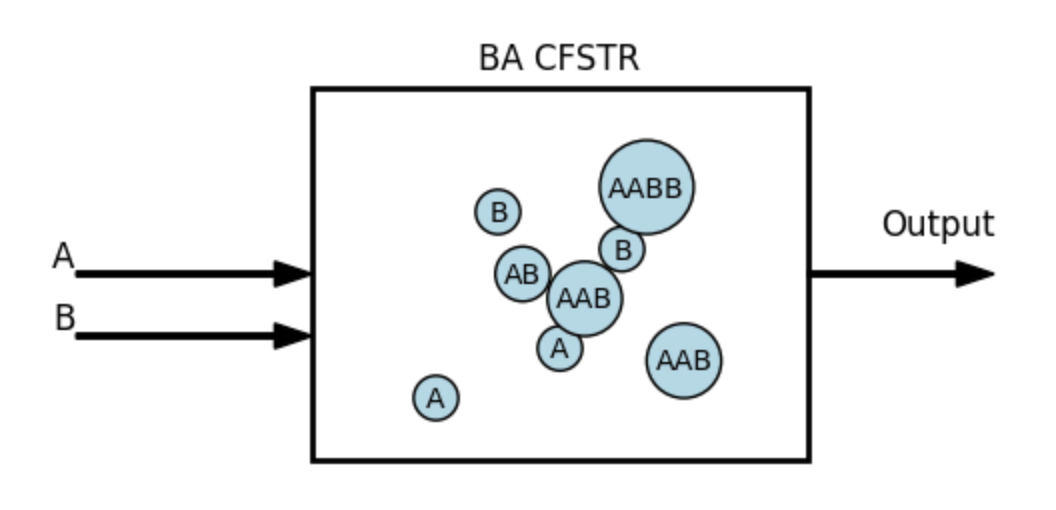
\includegraphics[height=5cm]{figure_1}
    \caption{Discrete BA analogue of a chemical Continuous Flow Stirred Tank Reactor (CFSTR)}
    \label{fig:figure_1}
\end{figure}

Selection emerges naturally through the interplay of stability and probabilistic interactions. Consider a simple BA system starting with a few instances of base elements \( A \) and \( B \). The pattern \( AB \) has a lifetime of 10 generations, while \( ABAB \) has a lifetime of 50 generations, and all other compounds degrade instantly with a lifetime of 0. After the first generation, the system produces combinations such as \( AA \), \( BB \), and \( AB \). Since \( AA \) and \( BB \) are unstable, they are eliminated, leaving \( A \), \( B \), and \( AB \). In subsequent generations, new unstable patterns may appear transiently, but \( AB \) persists due to its longer lifetime. Over time, the population of \( AB \) increases probabilistically, as multiple instances of \( AB \) are likely to form, increasing the likelihood of forming \( ABAB \). This dynamic reflects a form of roulette wheel selection \cite{goldberg1989genetic} \cite{holland1975adaptation}, where the stability-driven persistence of \( AB \) amplifies its probability of interaction. The emergent pattern \( ABAB \) represents a higher-order configuration, demonstrating how selection, grounded in differential stability, shapes the system's evolutionary pathways. The mechanism relies on the stability-induced bias in interaction probabilities, ensuring that patterns with greater persistence are favored, enabling the accumulation of complexity over successive generations.

The following simulation shows a different BA system with a population of 3 elements: {A, B, C}. Assume B-compounds are more stable than those without B. Thus patterns like BB, AB, BC, ABC, have a higher stability than AC or A or C. Therefore, B compounds will persist for multiple generations, while the others will quickly dissipate. The more stable B-compounds will interact more frequently due to their relative frequency, even though there is no replication or inheritance at the individual compound level. A snapshot of the simulation is shown in Figure \ref{fig:figure_2}.

\begin{figure}[htp]
    \centering
    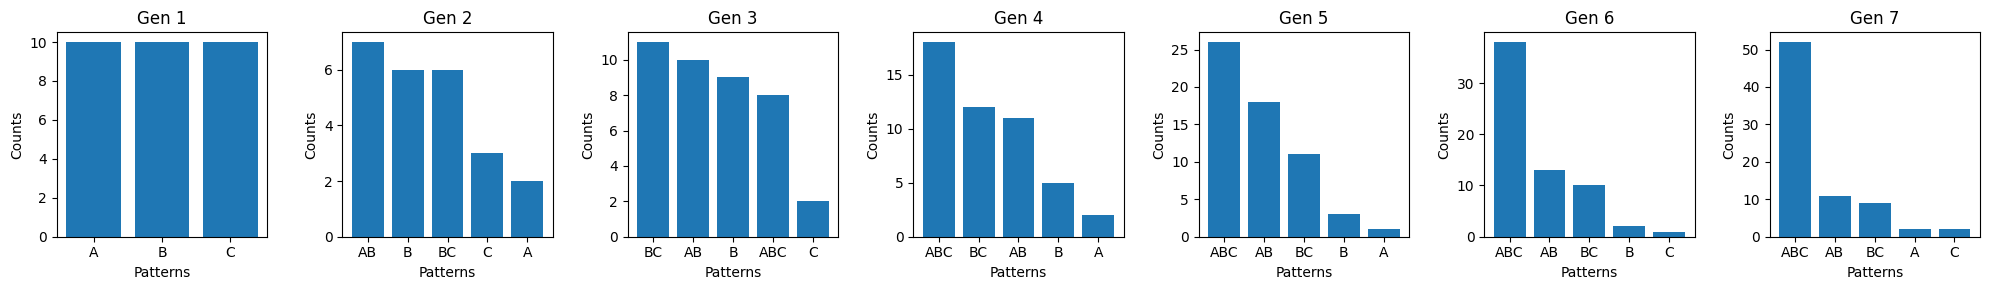
\includegraphics[width=1\textwidth]{figure_2}
    \caption{BA System population evolution simulation}
    \label{fig:figure_2}
\end{figure}

Where is Maxwell's demon \cite{leff2002maxwell} hiding in Figure \ref{fig:figure_2}, driving it towards a low-entropy state? As we saw, the answer lies in the roulette wheel. Compounds that persist longer have more chances to interact. As their frequency in the population increases, their chances to interact grow even more. In Evolutionary Dynamics, this is called fitness-proportionate selection \cite{back1996evolutionary} or roulette wheel selection \cite{goldberg1989genetic} \cite{holland1975adaptation}.

\section{Dual Probability Distributions Governing BA Systems}

BA systems can be effectively described by two interdependent probability distributions: the \textbf{population distribution}, which represents the relative abundance of patterns in the system, and the \textbf{stability distribution}, which quantifies the stable lifetime of successful compounds. The population distribution reflects the probabilities of patterns in any given generation \( t \). Let \( P_t(p) \) represent the probability of the pattern \( p \) in the population at time \( t \):
\[
P_t(p) = \frac{N_t(p)}{\sum_{q \in P} N_t(q)}
\]
where \( N_t(p) \) is the absolute count of pattern \( p \) in the population at time \( t \), and \( \sum_{q \in P} N_t(q) \) is the total population size at time \( t \), ensuring normalization (\( \sum_{p \in P} P_t(p) = 1 \)). The population distribution evolves over generations as patterns interact and new stable configurations emerge. As patterns with higher stability and frequent interactions become more prominent in the population, the population distribution evolves to reflect the history of past interactions and selection pressures.

The stability distribution \( S(p) \) represents the persistence or longevity of the individual pattern \( p \) in the system, defined as the expected lifetime or persistence of \( p \) over generations. Stability is a measure of how long a pattern remains viable before it dissipates or is replaced, reflecting physical properties such as energy barriers, bond strengths, environmental effects, and resistance to degradation.

Stability influences the dynamics of the system by determining how long a pattern persists to participate in future interactions. Patterns with higher stability values \( S(p) \) are more likely to accumulate over generations, increasing their representation in the population and increasing the likelihood of forming new patterns. This persistence-driven selection creates a feedback loop, where stable patterns dominate the system dynamics, guiding the evolution of complexity. 

In simulations of real-world scenarios, the values of \(S(p)\) would reflect the underlying physical, chemical, or even economic or social principles. In a chemical context, for example, these stability factors might be derived from binding energies, reaction rate constants, or free energies of formation. In an economic model, they could represent relative cost efficiencies or market resilience. In each case, \(S(p)\) encodes the notion of persistence in the relevant domain: the likelihood that a given compound, pattern, or agent survives long enough to interact and persist into the next generation. Unlike the population distribution, which evolves dynamically based on interactions, the stability distribution remains constant or changes only gradually. 

\subsection{Compound Persistence and Creation}

The probability of a pattern at generation \(t+1\) arises from two distinct processes:
\emph{persistence} of existing patterns and \emph{creation} of new copies. First, if a pattern \(p\) already exists at time \(t\), its ability to survive depends on its \emph{stability}:
\begin{equation}
\label{eq:persist-term}
\mathrm{Persist}_t(p) 
\;=\; 
P_t(p)\,\cdot\,S_t(p).
\end{equation}
Here, \(P_t(p)\) is the pattern's probability at generation~\(t\), and \(S_t(p)\) denotes its stability (expected lifetime). A higher \(S_t(p)\) increases the likelihood that \(p\) lasts or even grows in abundance from generation to generation. Second, more copies of pattern \(p\) can be \emph{created} through concatenations of other patterns:
\begin{equation}
\label{eq:create-term}
\mathrm{Create}_t(p)
\;=\;
\sum_{(q,r)\,\to\,p}\;P_t(q)\,P_t(r),
\end{equation}
where the notation \(\,(q,r)\to p\) indicates that \(p\) forms from combining patterns \(q\) and \(r\). This term captures how new copies of \(p\) appear whenever its reactants \(q\) and \(r\) are sufficiently probable within the population. For example, if there are copies of $AB, A, BA$ in the population, then $ABA$ can be formed by: $AB + A \to ABA$ or $A + BA \to ABA$. 

To obtain the final probability distribution at generation \(t+1\), we \emph{normalize} these contributions across all patterns:
\begin{equation}
\label{eq:full-ba-update}
P_{t+1}(p)
\;=\;
\frac{
  \mathrm{Persist}_t(p)
  \;+\;
  \mathrm{Create}_t(p)
}{
  \displaystyle \sum_{p'} 
  \Bigl[
    \mathrm{Persist}_t(p')
    \;+\;
    \mathrm{Create}_t(p')
  \Bigr]
}.
\end{equation}
Patterns with higher stability \(S_t(p)\) can retain a large share of the population (persistence), and patterns whose precursors \((q,r)\) are abundant can quickly emerge (creation). High initial abundance \(P_t(p)\) also confers an “inertial” advantage by multiplying with \(S_t(p)\). Conversely, novel patterns can claim probability mass through pairwise formation if \(q\) and \(r\) are sufficiently probable.

\subsection{Entropy Dynamics in BA Systems}

When we leave out the normalization constant in Equation~\ref{eq:full-ba-update} it becomes evident that two competing processes determine how the probability shifts across patterns:
\begin{equation}
P_{t+1}(p) \;\propto\; \mathrm{Persist}_t(p) \;+\; \mathrm{Create}_t(p).
\end{equation}
The $\mathrm{Persist}_t(p)$ term, defined by $P_t(p)\,S(p)$, grows sharply when $S(p)$ is large, concentrating probability in stable patterns and lowering entropy by making the distribution more peaked. Conversely, the $\mathrm{Create}_t(p)$ term, derived from $\sum_{(q,r)\to p}P_t(q)\,P_t(r)$, lets new or previously rare patterns emerge if their precursors $q$ and $r$ remain abundant, thus dispersing probability and raising entropy.

One may draw an analogy to a predator–prey dynamic: stable compounds act like predators by capturing and retaining probability at the expense of less stable patterns, while ephemeral or newly created compounds behave like prey by diffusing the distribution. In an unconstrained system without stability, there is no carryover advantage, so probability remains evenly spread and maintains high entropy. In a Bayesian Assembly (BA) system, however, sufficiently large-stability patterns typically outcompete the rest. If their cumulative effect exceeds the diversification introduced by creation events, the system’s entropy declines over time, ultimately settling into a low-entropy configuration dominated by a small number of robust patterns.

\section{Mixing Two BA Systems}

Mixing two independently evolved Bayesian Assembly (BA) systems introduces a new layer of complexity, where patterns and interactions from each system influence and reshape one another. This interaction results in the exchange of information, changes in entropy dynamics, and the emergence of novel patterns that were inaccessible within isolated systems.

Consider two independently evolved BA systems, each representing populations of compounds derived from distinct base elements: \( A, B, C, \dots \) for the first system and \( X, Y, Z, \dots \) for the second. Each system evolves separately, guided by its population distribution and node stability constraints. Upon mixing, the systems form a joint network, in which patterns from both systems interact to create compounds between systems (e.g., \( ABXX, BBYZ \)). Stability constraints, which govern the persistence of patterns, extend to these intersystem interactions, creating a dynamic interplay that determines the joint system's evolution. The updated probabilities in the combined system reflect both the within-system interactions and the newly formed cross-system interactions, as depicted in Figure~\ref{fig:figure_3}.

\begin{figure}[htp]
    \centering
    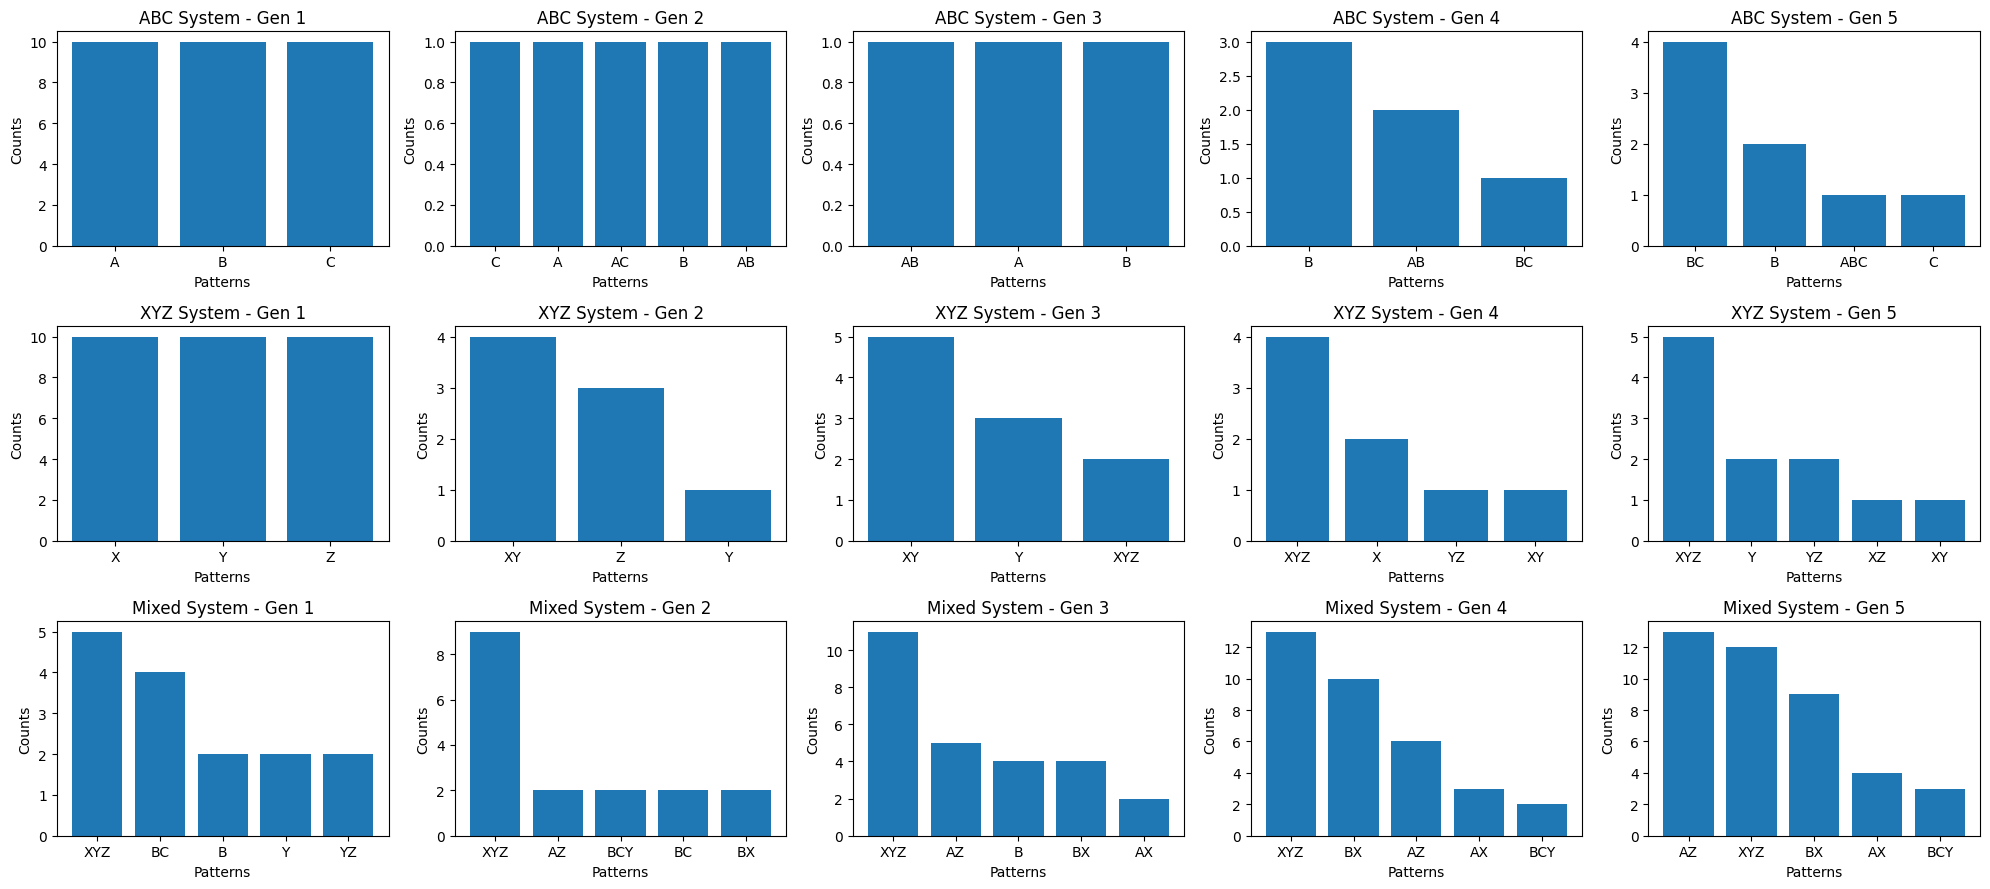
\includegraphics[width=13cm]{figure_3}
    \caption{Mixing two independently evolved populations in a Bayesian Assembly system. Cross-system interactions enable the emergence of novel compounds with high stability, fostering a broader exploration of the state space.}
    \label{fig:figure_3}
\end{figure}

An analogous process occurs in a continuous-flow stirred tank reactor (CFSTR) \cite{fogler1999chemical}, where two distinct chemical feeds are mixed to produce a steady-state mixture. Within this reactor, reactants from each feed can participate in cross-reactions, occasionally generating novel compounds (e.g., \( AZ \)) that exhibit greater stability than those found in either feed alone. This analogy underscores the role of cross-system interactions in driving emergent behavior and enhancing system complexity.

In the context of BA systems, mixing introduces a larger combined state space, where the stable patterns that evolved independently within each system now have increased opportunities to cross-interact. High-stability patterns from these cross-interactions proliferate over less stable alternatives, driven by stability feedback mechanisms.

\section{Bayesian Dynamics of Evolving Probability Distributions}

The evolving probability distribution in Bayesian Assembly (BA) systems can be understood through Kauffman's \emph{Theory of the Adjacent Possible} \cite{kauffman2000investigations, kauffman2024tap}, which describes how new states become accessible as existing structures form. In BA systems, patterns with higher stability persist and proliferate across generations, while less stable configurations dissipate. This iterative process allows the emergence of novel patterns in generation \( t+1 \) that were previously inaccessible in generation \( t \), driven by stability-weighted selection.

In an unconstrained system, newly formed patterns reset to uniform probabilities each generation, preventing any long-term bias. In contrast, BA systems evolve according to Equation \ref{eq:full-ba-update}, which can be written as:
\begin{equation}
P_{t+1}(p) \propto \underbrace{P_t(p)\,S(p)}_{\text{Persist}(p)} + \underbrace{\sum_{(q,r)\to p} P_t(q)\,P_t(r)}_{\text{Create}(p)},
\end{equation}
where \( \text{Persist}(p) = P_t(p) S(p) \) represents the survival of an existing pattern, akin to a Bayesian prior weighted by a stability-based likelihood. The second term, \( \text{Create}(p) \), accounts for the combinatorial formation of new copies of $p$ from precursor interactions.

This process parallels Bayesian updating: the prior distribution \( P_t(p) \) is modified by stability-weighted persistence and new combinatorial interactions, yielding a posterior distribution \( P_{t+1}(p) \) that governs the next generation. Unlike static Bayesian inference, where a fixed dataset refines a probability estimate, BA systems dynamically reshape their state space, allowing for genuine emergence. The frequentist probability of patterns within a generation reflects observed occurrences, but transitions between generations follow an evolving Bayesian update, demonstrating how stability-driven selection and probabilistic interactions drive the system toward structured complexity \cite{le2020equation}.

\subsection{Do BA Systems Truly Evolve?}

A natural question arises: do BA systems genuinely evolve, or is "evolution" merely an analogy? While BA systems lack explicit self-replication at the level of individual instances of a pattern $p_i$, they exhibit population-level dynamics that are mathematically indistinguishable from classical evolutionary processes. The fundamental mechanism driving this behavior is that more copies of $p$ are sustainably created from precursor patterns, leading to an increasing relative abundance $N_p$ in the population. This, in turn, grants $p$ more opportunities to participate in subsequent reactions, reinforcing its presence over generations. Moreover, the stability function $S(p)$ ensures that higher-stability patterns persist longer before being degraded or replaced, further amplifying their representation. These dynamics align precisely with the principles of fitness-weighted selection in evolutionary systems, where persistence and reproductive opportunity drive the emergence of dominant patterns. Since the probability of $p$'s continued presence is explicitly governed by its relative abundance and stability in a roulette-wheel selection process, we assert that BA systems exhibit genuine evolutionary behavior—not as a mere analogy, but as a mathematical inevitability.


\section{Stability Imbalances in Nature}

The abstract BA model is motivated by the universe’s vast stability disparities, from fleeting nuclear states to gravitationally bound structures lasting billions of years. These variations in binding energy, environmental interactions, and system resilience may dictate the formation and persistence of low-entropy structures, from molecular networks to planetary systems. Covalent bonds gain longevity in extended lattices like diamond and graphene, while geological formations evolve over millions of years under pressure and erosion. On cosmological scales, gravitationally bound systems, including planetary and galactic structures, persist across epochs, underscoring the fundamental role of stability in natural organization.

Beyond simple bond strength, the persistence of structures is influenced by factors such as spatial arrangements, catalytic reinforcement, feedback loops, and hierarchical assembly. Biological molecules, for instance, often derive stability not merely from strong covalent bonds but also from folded conformations, cooperative interactions, and self-repair mechanisms. Similarly, geological formations maintain their integrity over deep time due to self-reinforcing stress distributions and dynamic equilibrium with their environment. Table~\ref{tab:binding-forces} summarizes a broader range of stability-driven phenomena, highlighting their characteristic strengths and lifetimes across multiple scales.


\begin{table}
\centering
\caption{Representative Stability Mechanisms in Nature and Their Typical Lifetimes.}
\label{tab:binding-forces}
\begin{tabular}{l l}
\toprule
\textbf{Mechanism} & \textbf{Typical Lifetime} \\
\midrule
Weak Nuclear (Beta Decay) & $\mu$s to minutes \\
Strong Nuclear (Stable Nuclei) & Millions to trillions of years \\
Covalent Bonds (Organic Molecules) & Seconds to billions of years \\
Hydrogen Bonding (DNA, Proteins) & Picoseconds to seconds \\
Ionic Bonds (Salts, Minerals) & Seconds to millennia \\
Geological Structures (Mountains) & Thousands to billions of years \\
Gravitational Systems (Planets, Stars) & Millions to billions of years \\
\bottomrule
\end{tabular}
\end{table}

Table \ref{tab:binding-forces} illustrates how stability is not solely a function of bond strength but arises from evolved hierarchical structures, environmental effects, and self-reinforcing dynamics. In a BA system, high-stability patterns accumulate over generations, biasing the reaction landscape towards configurations that persist. This provides a simplified conceptual model for understanding how long-lived low-entropy structures emerge in nature through differential stability selection, whether in chemical systems, geological formations, or cosmic architecture.

\section{Simulation of Bayesian Assembly and Unconstrained Systems}

Unconstrained systems allow all possible compounds to form with equal likelihood each generation, leading to a combinatorial expansion of the state space. Let $N_t$ be the total number of compounds present in generation $t$. The probability of observing a specific compound $p$ can be approximated by $P_t(p) = \frac{1}{N_t}$. As $t$ increases, $N_t$ grows combinatorially, so $P_t(p) \to 0$ for any single compound. This uniform dispersion implies that no pattern dominates. Entropy in such a system typically remains high or increases as more compounds enter the state space.

To compare the dynamics of unconstrained and BA systems, we developed a simulation framework that models the evolution of compound formation over successive generations. This framework captures the key contrasts between the two regimes: the uniform expansion of state space of the unconstrained system and the stability-driven selection pressures of the BA system. The simulation begins with an initial population of base elements and proceeds through a fixed number of generations. The following pseudocode captures the main steps and shows that the only difference between the unconstrained and BA systems is in setting expiration times for compounds based on their stability:

\begin{center}
\begin{minipage}{0.9\textwidth}
\ttfamily
\begin{verbatim}
Initialize population with base elements
For each generation:
    Replenish base elements in population
    For each interaction:
        Randomly select a pair of elements from population
        Form compound by concatenation and add to population
        If BA system:
            Set compound expiration based on S(p)
    Remove expired elements from population
    Compact patterns into simplified representations
    Store population data for analysis
\end{verbatim}
\end{minipage}
\end{center}
The simulation results confirm that the unconstrained system disperses its probabilities over an expanding set of compounds, mirroring a uniform exploration of the combinatorial high-entropy state space. In contrast, the BA system channels probability into a subset of stable compounds. High-stability patterns become attractors, reducing entropy as the system evolves. Figure~\ref{fig:simulation_results} illustrates these differences: while the unconstrained distribution remains broad and diffuse, the BA distribution skews heavily toward stable patterns.

\begin{figure}[h]
    \centering
    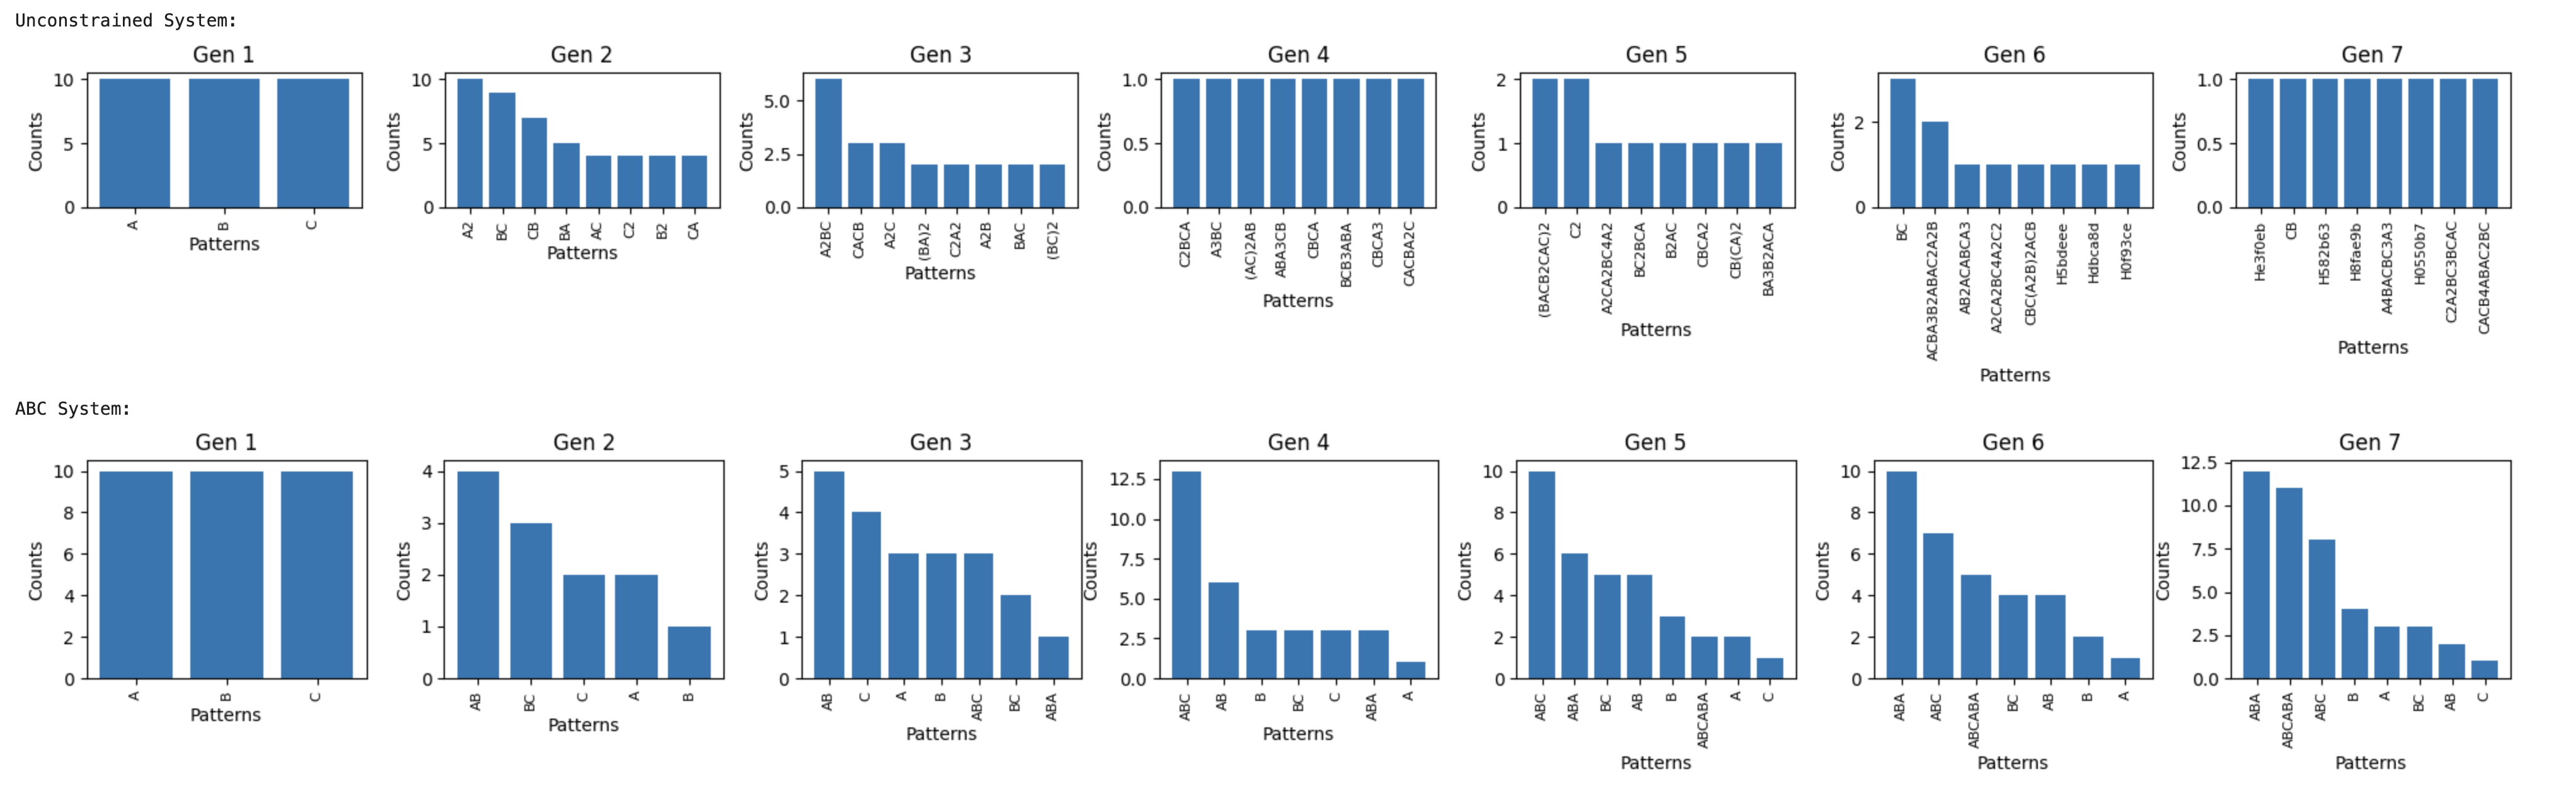
\includegraphics[width=1\textwidth,height=7cm]{figure_4.png}
    \caption{Comparison of the evolution of the unconstrained system and the BA system. 
    The unconstrained system exhibits a uniform distribution expanding over the state space, 
    whereas the BA system creates more copies of high-stability patterns, 
    thereby inducing order and reducing entropy.}
    \label{fig:figure_4}
 \end{figure}

\section{Dynamic Graph Representation and Token Flow Analysis}

To further investigate the dynamics of BA systems, we represent the state of the system in a specific generation as a directed graph, where the nodes correspond to base elements and compounds like $A$, $AB$, $ABA$, $ABC$, and the directed edges represent the interactions that occurred between them in their assembly process. Recall that the base elements $A$, $B$, $C$ are replenished in each generation, initiating a cascade of interactions that propagate "tokens" (shown in Figure~\ref{fig:figure_5} as the count $N$ of instances or copies of each pattern). Tokens represent the number of copies or instances of each pattern or compound at any generation, providing a direct measure of their relative population. Token flow describes the redistribution of these tokens across nodes in the reaction graph, driven by stability dynamics and interactions. This process is analogous to probability currents in quantum mechanics \cite{feynman1965quantum} and optimal transport \cite{villani2008optimal}, reflecting the macroscopic evolution of the system. The tokens accumulate at nodes based on the flow dynamics, which are governed by the stability of each pattern (shown in Figure~\ref{fig:figure_5} as $S$), influencing the persistence and selection of patterns over successive generations.


\begin{figure}[h]
    \centering
    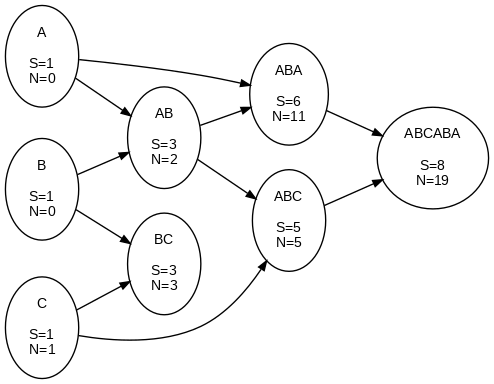
\includegraphics[width=0.7\linewidth]{figure_5.png}
    \caption{Graph representation of a BA system showing stability (S), and the number of instances or tokens (N) of each base element and compound.}
    \label{fig:figure_5}
\end{figure}

The dynamic graph in Figure~\ref{fig:figure_5} represents the 7th generation of the simulation shown in Figure~\ref{fig:figure_4}. The distribution of tokens across the graph reveals insights into the self-reinforcing nature of stability in BA systems. Nodes with higher stability values (\textit{e.g.}, $ABCABA$) attract more tokens, leading to the emergence of dominant patterns. This phenomenon reflects a feedback loop: As tokens accumulate at a stable node, it becomes increasingly likely to dominate subsequent interactions, establishing preferential flow paths through the graph. Consequently, the system's token traffic converges to well-defined routes, concentrating resources on a subset of high-stability patterns while marginalizing less stable ones.

However, the graph may change significantly between generations if a new disruptor node emerges in the system. A disruptor node is characterized by a high stability value and strategic positioning within the graph, enabling it to compete with previously dominant nodes for token traffic. This disruptor can reroute flows, effectively redistributing tokens and breaking established dominance patterns. 

From a physical perspective, the behavior of token flows in the BA system parallels physical phenomena such as those observed in fluid systems, where a new high-conductivity channel can divert flow away from existing pathways. Similarly, in RC circuits, the introduction of a new low-resistance branch redistributes the current, altering the overall system equilibrium. 

Dynamic graphs have been used for switch-level simulation of transistor networks \cite{AdlerCAD}, where graph pathways are dynamically determined by the state of the on transistors, enabling specific connections to guide current flow. Similarly, in BA systems, token flow is governed by stability and probabilistic interactions, determining which nodes persist and propagate.

\subsection{Chemical Example: Iron Oxidation}

\begin{figure}[h]
    \centering
    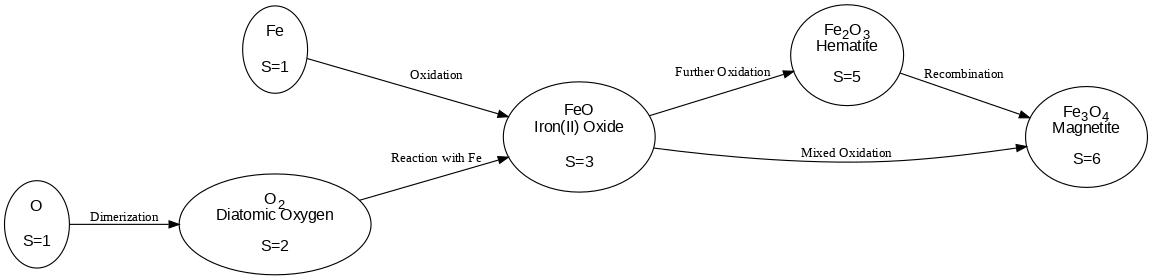
\includegraphics[width=1\textwidth,height=0.4\textwidth]{figure_6.png}
    \caption{Reaction network for iron oxidation, illustrating the stepwise formation of stable and intermediate compounds under stability constraints.}
    \label{fig:figure_6}
\end{figure}

The principles of Bayesian Assembly (BA) systems can be illustrated through the oxidation of iron, a realistic and naturally occurring chemical process. As shown in Figure~\ref{fig:figure_6}, the oxidation of iron (\(Fe\)) proceeds through a network of reactions driven by stability constraints. Oxygen (\(O\)) forms diatomic oxygen (\(O_2\)), which reacts with iron to produce a series of oxides, including iron(II) oxide (\(FeO\)), iron(III) oxide (\(Fe_2O_3\), hematite), and iron(II,III) oxide (\(Fe_3O_4\), magnetite). These reactions represent a progression from less stable intermediates to thermodynamically favored compounds. Competing pathways, such as partial oxidation or the formation of unstable intermediates, illustrate how stability shapes the evolution of the system, favoring reactions that lead to more persistent and energetically favorable products.

In the BA framework, node stability \(S(p)\) quantifies the persistence of each compound, with higher stability values assigned to products like hematite and magnetite due to their robust bonding and lower susceptibility to dissociation. This reaction network provides a testable system for validating the role of stability in driving reaction pathways. By simulating token flow dynamics based on stability values, the framework captures how high-stability compounds emerge and dominate over successive generations, aligning with experimental observations of oxidation processes.


\subsection{Organic Chemistry Examples and Their BA System Interpretations}
\label{sec:organic-ba-examples}

Two reaction graphs from organic chemistry provide illustrative cases for understanding how Bayesian Assembly (BA) systems can model complex pathways at a high level. Although neither example specifically reflects a continuous-flow stirred tank reactor (CFSTR), both showcase how the concept of node stability can guide the formation and persistence of certain molecular arrangements. By assigning relative stability values to each species based on physical and chemical considerations, one can track how the resulting population of intermediates evolves according to the generational dynamics of BA systems.

\begin{figure}[h]
    \centering
    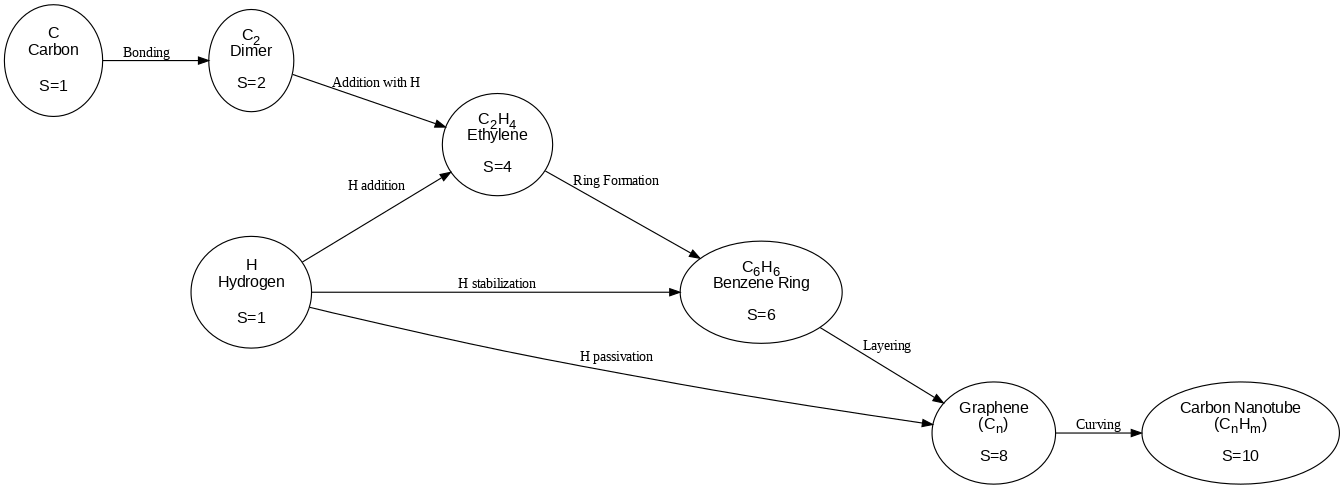
\includegraphics[width=1\textwidth,height=0.55\textwidth]{figure_7.png}
    \caption{Reaction graph for possible Carbon Nanostructure Assembly}
    \label{fig:figure_7}
\end{figure}

Figure~\ref{fig:figure_7} illustrates an abstract reaction graph showing the progressive assembly of carbon-based structures, starting from simple carbon monomers (\( \text{C} \)) and hydrogen atoms (\( \text{H} \)). In the early stages, carbon atoms bond to form dimers (\( \text{C}_2 \)) or small hydrocarbons like ethylene (\( \text{C}_2\text{H}_4 \)). Through additional interactions and stabilization processes, these smaller molecules transition into increasingly complex structures, such as benzene (\( \text{C}_6\text{H}_6 \)), which serves as a precursor for planar graphene sheets (\( \text{C}_n \)). Ultimately, graphene sheets curl into carbon nanotubes (\( \text{C}_n\text{H}_m \)), high-stability configurations characterized by their exceptional mechanical and electrical properties. 

The main pathway emphasizes the gradual increase in structural complexity and stability. Alongside this progression, less stable intermediates, such as defective graphene or transient molecules, may arise but typically do not persist due to lower stability. These transient species reflect pathways that are accessible in the reaction space but are pruned over successive iterations. Here, stability \( S(p) \) plays a central role in determining the persistence and influence of each compound. Simple elements (\( \text{C} \), \( \text{H} \)) and early products (\( \text{C}_2 \), \( \text{C}_2\text{H}_4 \)) possess baseline stability values, representing their shorter lifetimes and higher turnover rates. As more complex compounds form, their stability parameters increase, reflecting stronger bonding, lower dissociation rates, and greater resistance to perturbation. Generational updates in a BA model dynamically favor the accumulation of these high-stability patterns, leading to the dominance of advanced nanostructures. In contrast, low-stability pathways fade over time, illustrating how stability-driven selection sculpts the molecular landscape and guides the emergence of ordered, complex systems.


\begin{figure}[h]
    \centering
    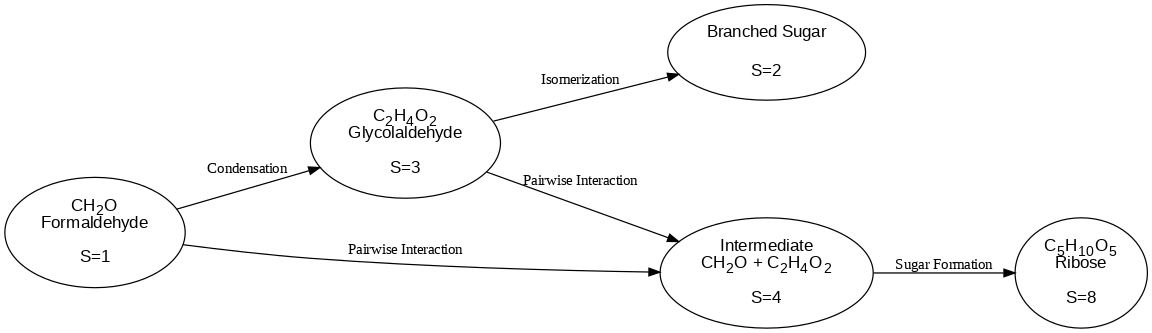
\includegraphics[width=1\textwidth,height=0.4\textwidth]{figure_8.png}
    \caption{Reaction graph for possible pre-RNA Sugar Assembly}
    \label{fig:figure_8}
\end{figure}

Figure~\ref{fig:figure_8} illustrates a simplified reaction network where small carbonyl-containing molecules, such as formaldehyde (CH$_2$O), undergo pairwise interactions to form sugars of increasing complexity. The pathway begins with the condensation of formaldehyde into glycolaldehyde (C$_2$H$_4$O$_2$), which can interact further to form intermediate compounds, such as a dimer of formaldehyde and glycolaldehyde. These intermediates then serve as precursors to ribose (C$_5$H$_{10}$O$_5$), a key sugar and a crucial building block for RNA. Alongside the main reaction pathway, side reactions lead to the formation of less stable by-products, such as branched sugars, which typically dissipate due to their lower persistence.

In this Bayesian Assembly (BA) framework, stability $S(p)$ quantifies the likelihood that each compound persists over successive reaction cycles. Ribose, for instance, achieves a high stability once formed, enabling its accumulation over generations. By contrast, transient intermediates and less stable by-products, such as branched sugars, quickly dissipate and contribute minimally to the evolving population. 

These two examples from organic chemistry highlight how stability may play a key role in complex reaction graphs. The BA perspective supplements conventional kinetic modeling by focusing on net generational outcomes and selective retention, rather than detailing every reversible step. In doing so, BA systems reveal how certain ``attractor'' molecules or assemblies can emerge in an otherwise large and branching reaction space, reinforcing the view that stability-driven selection is a powerful force in shaping molecular evolution.

\subsection{Mass Action Kinetics and Forward-Generation Constraints}
\label{subsec:mak-forward-limitations}

Mass Action Kinetics (MAK) \cite{TuranyiTomlin2014} provides deterministic rate equations for chemical reactions, such as
\[
\frac{d[A]}{dt} \;=\; -\,k\, [A]\,[B],
\]
where $[A]$ and $[B]$ represent concentrations and $k$ is a rate constant. These equations capture conservation laws for mass and energy and can reflect selection processes under certain conditions. More recent work such as Chemical Organization Theory (COT) \cite{DittrichFenizio2005} emphasizes the finding of closed and self-maintaining collections of species in a fixed reaction network. Assembly Theory (AT) has proposed the use of MAK-like forward models to link object production to assembly indices and copy numbers \cite{walker2023nature}.

MAK inherently allows reactions to run both forward and backward with fixed-rate laws, posing a challenge for assembly frameworks like AT and BA that emphasize net forward construction. Although MAK excels at describing known reaction networks under equilibrium or near-equilibrium assumptions, it lacks a mechanism for the open discovery of novel compounds central to BA’s approach.

\subsection{Analogy to Electronic Circuit Simulations}
\label{subsec:spice-analogy}

In MAK models species concentrations evolve as 
$\dot{\mathbf{x}} = \mathbf{A}\,\mathbf{x} + \mathbf{b}$, where \(\mathbf{x}\) represents species concentrations, \(\mathbf{A}\) encodes stoichiometric and kinetic-rate constants, and \(\mathbf{b}\) accounts for base-element replenishment, driving the system away from thermodynamic equilibrium. A similar formulation appears in electronic circuit simulation, where node voltages evolve as 
$\dot{\mathbf{v}} = \mathbf{A}\,\mathbf{v} + \mathbf{b}$, with \(\mathbf{A}\) capturing conductances and small-signal transistor gains, and \(\mathbf{b}\) representing external sources. These models resolve bidirectional flows and fine-grained transient dynamics at each time step.

Higher-level abstractions, such as switch-level simulation \cite{AdlerCAD}, forego solving the full system of ODEs, instead tracking discrete state transitions. At an even coarser gate level \cite{FeynmanComp}, circuits are modeled as idealized logical operations, discarding continuous voltage dynamics.

BA systems adopt a similarly abstracted perspective: rather than modeling bidirectional reaction flows explicitly, they capture dominant generational updates, analogous to switch- or gate-level simulation in circuits. Stability-driven selection replaces continuous-time reversibility, focusing on net forward assembly steps that determine the persistence and evolution of patterns.

\subsection{Economic Example: Industry Ecosystem as a BA System}

This example illustrates a Bayesian Assembly (BA) system applied to an economic context, where base elements represent different types of businesses. Manufacturers (A), retailers (B), and logistics providers (C) act as base elements with stabilities \( S_A, S_B, S_C \) reflecting their persistence in the market. Through successive interactions, these base elements form partnerships \( AB \), \( AC \), \( BC \) and evolve into integrated networks \( ABAC \), \( ABBC \), as shown in Figure~\ref{fig:figure_9}. Each stage corresponds to increasingly complex collaborations, where stability-driven selection ensures the persistence of dominant nodes. 

\begin{figure}[h]
    \centering
    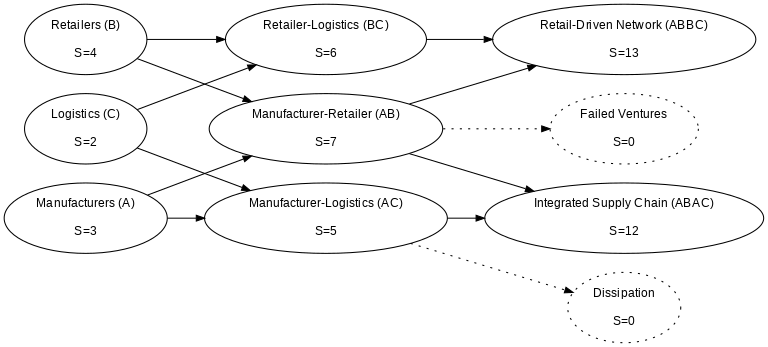
\includegraphics[width=1\textwidth]{figure_9.png}
    \caption{Industry ecosystem represented as a BA system, showing the evolution from base businesses (\( A, B, C \)) to partnerships and stable integrated networks (\( ABAC, ABBC \)).}
    \label{fig:figure_9}
\end{figure}

Stable nodes, such as \( AB \) (manufacturer-retailer) and \( ABBC \) (retail-driven networks), act as attractors, accumulating resources (tokens) over generations. Less stable nodes, including failed ventures (\( S=0 \)), dissipate quickly, redistributing tokens to more viable configurations. This process mirrors the dynamics of BA systems, where selection amplifies stable patterns and suppresses randomness, driving the emergence of structured, low-entropy configurations. The economic analogy emphasizes how stability influences token flow, resource allocation, and the formation of hierarchical networks in complex systems. The tokens in this graph (individual companies) will naturally flow to configurations that are more stable and persistent, representing more business opportunities.

\section{Top-Down vs.\ Bottom-Up Dynamics in BA Systems}
\label{sec:topdown-bottomup}

Figure~\ref{fig:figure_10} illustrates the interplay between top-down and bottom-up causality in Bayesian Assembly (BA) systems, where the top-down influence emerges from the increasing relative abundance of stable patterns directing subsequent interactions, while bottom-up processes arise from the probabilistic assembly of base elements into intermediate and complex patterns, creating a dynamic feedback loop that drives the evolution of information and complexity.

\begin{figure}[h]
    \centering
    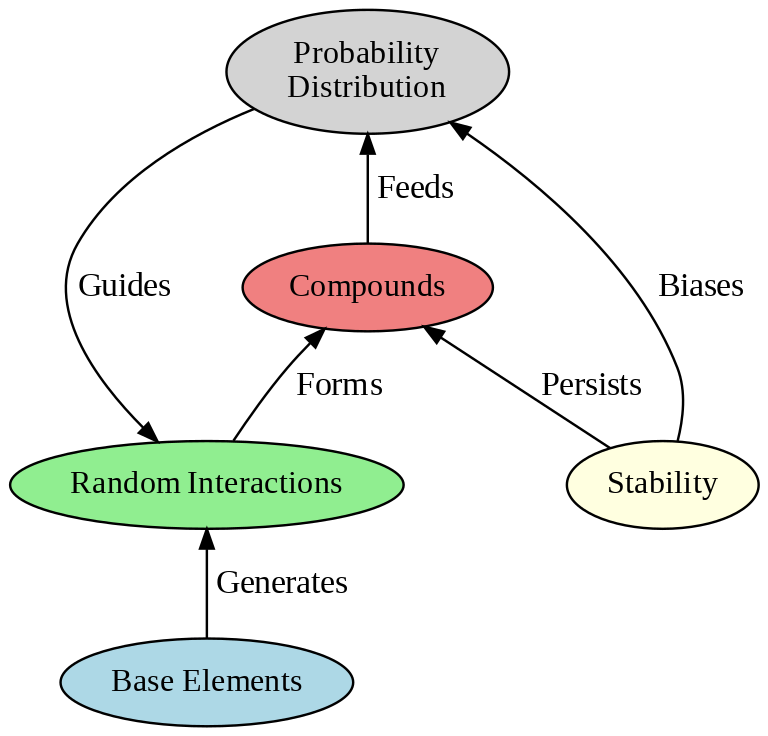
\includegraphics[width=0.7\linewidth,height=0.7\linewidth]{figure_10.png}
    \caption{Bottom-up and Top-down causality in BA systems}
    \label{fig:figure_10}
\end{figure}

Once certain patterns become dominant, they exert a top-down influence on subsequent generations. These higher-level persistent structures shape future interactions by catalyzing or constraining the formation of new patterns. Hence, BA systems do not just accumulate complexity through local rules; they also incorporate feedback from emergent structures that guide (or ``select for'') new configurations. The presence of memory and evolutionary history in these feedback loops distinguishes BA systems from frameworks in which higher-level states simply describe aggregates without influencing the underlying microstates.

The contrast with traditional statistical mechanics is striking \cite{landau1980statistical}. In statistical mechanics, macrostates (e.g., temperature, pressure) represent aggregate properties of microstates but do not directly influence the fundamental interaction rules among particles. In BA systems, however, dominant patterns exert a causal influence on micro-level interactions, embedding history and specificity into the generative process itself. This dynamic distinguishes BA systems by allowing feedback mechanisms that shape pattern evolution, independent of predefined energy distributions or equilibrium constraints.

Such an explicit interplay between bottom-up and top-down dynamics in BA systems suggests a broader principle for understanding complexity: emergent structures can become causal agents that direct further evolution of the system. This perspective helps explain the accumulation of novel order in contexts ranging from prebiotic chemistry to computational networks, where higher-level assemblies (compounds, motifs, or functional components) increasingly govern local interactions, thereby catalyzing the exploration of new possibilities for growth and adaptation.

At times, these dynamics appear teleological, as if the system were ``seeking'' more stable or more complex configurations. Bertalanffy \cite{bertalanffy1968general} cautions that such optimization processes, while suggestive of goal-directed behavior, often reflect nothing more than the natural unfolding of feedback loops and gradients rather than true purposeful design. BA systems likewise illustrate how feedback from emergent structures can drive the exploration of new system states without implying an external or predetermined goal. By capturing both bottom-up and top-down mechanisms in an evolving distribution, BA systems provide a model for understanding how complexity can accumulate, whether in prebiotic chemistry or in computational and informational domains, through iterative processes of selection and the continual reshaping of local interactions.


\section{Conclusion}

BA systems provide a simple framework for understanding the emergence of complexity and order in systems governed by probabilistic interactions and stability-driven selection. By abstracting away specific physical laws, these systems offer a testable and generalizable model applicable to a wide range of phenomena. 

The iterative interaction of elements in BA systems may help explain the evolution of matter and energy. From the aggregation of quarks into elementary particles, to the evolution of molecules and chemistry. The periodic table, for example, organizes elements based on properties such as ionization energy, chemical reactivity, etc. These properties bias element interactions, favoring stable configurations. For example, \( H_2 \) forms in dense regions of space where hydrogen atoms collide and bond. It is stable because of strong covalent bonds and serves as a building block for stars. This reflects the dominance of stability-driven patterns, akin to how BA systems reinforce stable patterns over generations. 

BA systems suggest that evolution may be a universal property of random populations with stability imbalances, not confined to living organisms. By demonstrating how random populations with stability-driven interactions naturally evolve toward order, this framework proposes that perhaps biological evolution of individual organisms is a later stage in such dynamics. Recent findings suggest that stability-driven self-assembly mechanisms may play a crucial role in biotic systems, highlighting the interplay between abiotic and biological evolution \cite{davies2022selfassembly}.

BA systems provide a non-mystical explanation of the origins of order and information, but they still leave open the question of fine-tuning. Fine-tuned imbalances, such as those described in Rees' \textit{Just Six Numbers} \cite{rees2000just} and Davies' \textit{The Goldilocks Enigma} \cite{davies2006goldilocks}, exemplify how asymmetries in fundamental constants enable complexity across scales. For instance, quantum fluctuations may have seeded the formation of stars and galaxies. Similarly, in BA systems,  non-uniform stability biases interactions toward forming persistent ordered patterns. This connection reinforces the idea that evolution, driven by imbalance and selection, operates universally, bridging the emergence of complexity from the cosmological to molecular scales. In summary, if the analogy holds and the universe turns out to evolve like a BA system, one might be tempted to say that God does indeed play dice, but the dice are loaded.


%\begin{listing}[H]
%\caption{Title of the listing}
%\rule{\columnwidth}{1pt}
%\raggedright Text of the listing. In font size footnotesize, small, or normalsize. Preferred format: left aligned and single spaced. Preferred border format: top border line and bottom border line.
%\rule{\columnwidth}{1pt}
%\end{listing}

%%%%%%%%%%%%%%%%%%%%%%%%%%%%%%%%%%%%%%%%%%
\vspace{6pt} 

%%%%%%%%%%%%%%%%%%%%%%%%%%%%%%%%%%%%%%%%%%
%% optional
%\supplementary{The following supporting information can be downloaded at:  \linksupplementary{s1}, Figure S1: title; Table S1: title; Video S1: title.}

% Only for journal Methods and Protocols:
% If you wish to submit a video article, please do so with any other supplementary material.
% \supplementary{The following supporting information can be downloaded at: \linksupplementary{s1}, Figure S1: title; Table S1: title; Video S1: title. A supporting video article is available at doi: link.}

% Only for journal Hardware:
% If you wish to submit a video article, please do so with any other supplementary material.
% \supplementary{The following supporting information can be downloaded at: \linksupplementary{s1}, Figure S1: title; Table S1: title; Video S1: title.\vspace{6pt}\\
%\begin{tabularx}{\textwidth}{lll}
%\toprule
%\textbf{Name} & \textbf{Type} & \textbf{Description} \\
%\midrule
%S1 & Python script (.py) & Script of python source code used in XX \\
%S2 & Text (.txt) & Script of modelling code used to make Figure X \\
%S3 & Text (.txt) & Raw data from experiment X \\
%S4 & Video (.mp4) & Video demonstrating the hardware in use \\
%... & ... & ... \\
%\bottomrule
%\end{tabularx}
%}

%%%%%%%%%%%%%%%%%%%%%%%%%%%%%%%%%%%%%%%%%%

\funding{This research received no external funding}

\institutionalreview{Not applicable}

\informedconsent{Not applicable}

\dataavailability{Not applicable} 

\acknowledgments{}

\conflictsofinterest{The author declares no conflicts of interest} 

%%%%%%%%%%%%%%%%%%%%%%%%%%%%%%%%%%%%%%%%%%
%%%%%%%%%%%%%%%%%%%%%%%%%%%%%%%%%%%%%%%%%%
%%%%%%%%%%%%%%%%%%%%%%%%%%%%%%%%%%%%%%%%%%
\begin{adjustwidth}{-\extralength}{0cm}
%\printendnotes[custom] % Un-comment to print a list of endnotes

\reftitle{References}

% Please provide either the correct journal abbreviation (e.g. according to the “List of Title Word Abbreviations” http://www.issn.org/services/online-services/access-to-the-ltwa/) or the full name of the journal.
% Citations and References in Supplementary files are permitted provided that they also appear in the reference list here. 

%=====================================
% References, variant A: external bibliography
%=====================================
%\bibliography{your_external_BibTeX_file}

%=====================================
% References, variant B: internal bibliography
%=====================================
\begin{thebibliography}{999}

%ref 1
\bibitem{schrodinger1944life}
Schrödinger, E. \textit{What is Life?}; Cambridge University Press: Cambridge, UK, 1944.

%ref 2
\bibitem{tegmark2008mathematical}
Tegmark, M. The Mathematical Universe. \textit{Found. Phys.} \textbf{2008}, \textit{38}, 101–150. 

%ref 3
\bibitem{fisher1930genetical}
Fisher, R.A. \textit{The Genetical Theory of Natural Selection}; Oxford University Press: Oxford, UK, 1930.

%ref 4
\bibitem{nowak2006evolutionary}
Nowak, M.A. \textit{Evolutionary Dynamics: Exploring the Equations of Life}; Belknap Press: Cambridge, MA, USA, 2006.

%ref 5
\bibitem{wheeler1990itbit}
Wheeler, J.A. Information, Physics, Quantum: The Search for Links. In \textit{Complexity, Entropy, and the Physics of Information}; Zurek, W.H., Ed.; Addison-Wesley: Redwood City, CA, USA, 1990; pp. 3–28.

%ref 6
\bibitem{noble2012causality}
Noble, D. A Theory of Biological Relativity: No Privileged Level of Causation. \textit{Interface Focus} \textbf{2012}, \textit{2}, 55–64.

%ref 7
\bibitem{lloyd2006programming}
Lloyd, S. \textit{Programming the Universe: A Quantum Computer Scientist Takes on the Cosmos}; Alfred A. Knopf: New York, NY, USA, 2006.

%ref 8
\bibitem{kolmogorov1965complexity}
Kolmogorov, A.N. Three Approaches to the Quantitative Definition of Information. \textit{Problemy Peredachi Informatsii} \textbf{1965}, \textit{1}, 3–11.

%ref 9
\bibitem{chaitin1977algorithmic}
Chaitin, G.J. Algorithmic Information Theory. \textit{IBM J. Res. Dev.} \textbf{1977}, \textit{21}, 350–359. 

%ref 10
\bibitem{solomonoff1964formal}
Solomonoff, R.J. A Formal Theory of Inductive Inference. Part I and Part II. \textit{Inf. Control} \textbf{1964}, \textit{7}, 1–22, 224–254.

%ref 11
\bibitem{shannon1948mathematical}
Shannon, C.E. A Mathematical Theory of Communication. \textit{Bell Syst. Tech. J.} \textbf{1948}, \textit{27}, 379–423.

%ref 12
\bibitem{deutsch2013constructor}
Deutsch, D.; Marletto, C. Constructor theory of information. \textit{Proceedings of the Royal Society A: Mathematical, Physical and Engineering Sciences} \textbf{2015}, \textit{471}, 20140540. 

\bibitem{walker2023nature}
S. I. Walker, L. Cronin, and others,
"Assembly theory explains and quantifies selection and evolution across physical and biological systems," \textit{Nature}, \textbf{618}, 619-628 (2023), doi:10.1038/s41586-023-06600-9.

\bibitem{kauffman2024tap}
M. Cortês and S.A. Kauffman and A.R. Liddle and L. Smolin (2024), "The TAP equation: evaluating combinatorial innovation in Biocosmology" arXiv:2204.14115


\bibitem{TuranyiTomlin2014}
Turányi, T., Tomlin, A. S. (2014). \textit{Analysis of Kinetic Reaction Mechanisms}. Springer. doi:10.1007/978-3-642-38516-1.

\bibitem{feinberg1987chemical}
Feinberg, M. (1987). Chemical Reaction Network Structure and the Stability of Complex Isothermal Reactors—I. The Deficiency Zero and Deficiency One Theorems. \textit{Chemical Engineering Science}, 42(10), 2229–2268. doi:10.1016/0009-2509(87)80099-4.

\bibitem{arxiv:q-bio0501016}
Gillespie, D. T. (2005). Stochastic Simulation of Chemical Kinetics. \textit{arXiv:q-bio/0501016}. Retrieved from https://arxiv.org/pdf/q-bio/0501016.

\bibitem{tononi2008phi}
Tononi, G. (2008). Consciousness as Integrated Information: A Provisional Manifesto. \textit{Biological Bulletin}, 215(3), 216–242. doi:10.2307/25470707.

\bibitem{fogler1999chemical}
Fogler, H. S. (1999). \textit{Elements of Chemical Reaction Engineering} (3rd ed.). Prentice Hall.

%ref 13
\bibitem{leff2002maxwell}
Leff, H.S.; Rex, A.F. \textit{Maxwell’s Demon: Entropy, Information, Computing}; Princeton University Press: Princeton, NJ, USA, 2002.

%ref 14
\bibitem{back1996evolutionary}
Bäck, T.; Fogel, D.B.; Michalewicz, Z. \textit{Evolutionary Computation 1: Basic Algorithms and Operators}; CRC Press: FL, USA, 2000.

%ref 15
\bibitem{goldberg1989genetic}
Goldberg, D.E. \textit{Genetic Algorithms in Search, Optimization, and Machine Learning}; Addison-Wesley: Boston, MA, USA, 1989.

%ref 16
\bibitem{holland1975adaptation}
Holland, J.H. \textit{Adaptation in Natural and Artificial Systems}; University of Michigan Press: Ann Arbor, MI, USA, 1975.

%ref 20
\bibitem{mcgrayne2011theory}
McGrayne, S.B. \textit{The Theory That Would Not Die: How Bayes' Rule Cracked the Enigma Code, Hunted Down Russian Submarines, and Emerged Triumphant from Two Centuries of Controversy}; Yale University Press: New Haven, CT, USA, 2011.

%ref 21
\bibitem{kauffman2000investigations}
Kauffman, S. \textit{Investigations}; Oxford University Press: New York, NY, USA, 2000.

\bibitem{le2020equation} N. Le, \textit{The Equation of Knowledge: From Bayes’ Rule to a Unified Philosophy of Science}, Philosophical Press, New York, NY, 2020.

\bibitem{DittrichFenizio2005}
P.~Dittrich and P.~S.~di Fenizio, ``Chemical organization theory: towards a theory of constructive dynamical systems,'' \emph{arXiv preprint arXiv:q-bio/0501016}, 2005.


\bibitem{SpiceRef}
L.~W.~Nagel and D.~O.~Pederson, ``SPICE (Simulation Program with Integrated Circuit Emphasis),'' 
{\em University of California, Berkeley}, Memorandum No. ERL-M382, Apr. 1973.

\bibitem{feynman1965quantum}
Feynman, R. P., \& Hibbs, A. R. (1965). \textit{Quantum Mechanics and Path Integrals}. McGraw-Hill.

\bibitem{villani2008optimal}
Villani, C. (2008). \textit{Optimal Transport: Old and New}. Springer Science \& Business Media.


\bibitem{AdlerCAD} D.~Adler, ``Switch Level Simulation Using Dynamic Graph Algorithms,''
{\em IEEE Transactions on Computer-Aided Design of Integrated Circuits and Systems}, vol.~10, March~1991.

\bibitem{FeynmanComp}
R.~P.~Feynman, {\em Feynman Lectures On Computation}, Westview Press, 1996.

%ref 22
\bibitem{landau1980statistical}
Landau, L. D., Lifshitz, E. M. \textit{Statistical Physics}; Pergamon Press, 1980.

%ref 23
\bibitem{bertalanffy1968general}
Bertalanffy, L. von. (1968). \textit{General System Theory}. New York: George Braziller.

%ref 25
\bibitem{davies2022selfassembly}
Davies, J.; Levin, M. Self-Assembly: Synthetic morphology with agential materials. \textit{Nature Reviews Bioengineering} v 1 (2023).

%ref 26
\bibitem{rees2000just}
Rees, M. \textit{Just Six Numbers: The Deep Forces that Shape the Universe}; Basic Books: New York, NY, USA, 2000.

%ref 27
\bibitem{davies2006goldilocks}
Davies, P. \textit{The Goldilocks Enigma: Why is the Universe Just Right for Life?}; Allen Lane: London, UK, 2006.


\end{thebibliography}

%% Add \usepackage{lineno} before \begin{document} and uncomment 
%% following line to enable line numbers
%% \linenumbers


\end{document}

\endinput
%%
%% End of file `elsarticle-template-num.tex'.
